\documentclass{ximera}

\begin{document}
	\author{Stitz-Zeager}
	\xmtitle{Exponential Functions}


\mfpicnumber{1}

\opengraphsfile{ExponentialFunctions}

\setcounter{footnote}{0}

\label{ExponentialFunctions}

Of all of the functions we study in this text, exponential  functions are possibly the ones which impact everyday life the most. This section introduces us to these functions while the rest of the chapter will more thoroughly explore their properties. 

\smallskip

 Up to this point, we have dealt with functions which involve terms like $x^3$,  $x^{\frac{3}{2}}$, or $x^{\pi}$ -  in other words, terms of the form  $x^{p}$ where the base of the term, $x$, varies but the exponent of each term, $p$, remains constant.  
 
 \smallskip
 
 In this chapter, we study functions of the form $f(x) = b^{x}$ where the base $b$ is a constant and the exponent $x$ is the variable.  We start our exploration of these functions with the time-honored classic,  $f(x) = 2^{x}$.  
 
 \smallskip
 
 We make a table of function values, plot enough points  until we are more or less confident with the shape of the curve,  and connect the dots in a pleasing fashion.

\hspace{1in} \begin{tabular}{m{2.7in}m{3in}}

\setlength{\extrarowheight}{4pt}
\[ \begin{array}{|r||r|r|}  

\hline

 x & f(x) & (x,f(x)) \\ \hline
-3 & 2^{-3} = \frac{1}{8} & \left(-3, \frac{1}{8} \right) \\ [2pt] \hline
-2 & 2^{-2} = \frac{1}{4} &  \left(-2, \frac{1}{4} \right) \\ [2pt] \hline
-1 & 2^{-1} = \frac{1}{2} &  \left(-1, \frac{1}{2} \right) \\ [2pt]  \hline
0  & 2^{0} = 1 & ( 0 ,1) \\  \hline
1  & 2^{1} = 2 & ( 1, 2) \\  \hline
2  & 2^{2} = 4 & (2,4) \\  \hline
3  & 2^{3} = 8 & (3, 8) \\  \hline
\end{array} \] 
\setlength{\extrarowheight}{2pt}

&

\begin{mfpic}[13]{-4}{4}{-1}{9}

\axes
\tlabel[cc](4,-0.5){\scriptsize $x$}
\tlabel[cc](0.5,9){\scriptsize $y$}
\tcaption{\scriptsize $y = f(x) = 2^{x}$}
\xmarks{-3,-2,-1,1,2,3}
\ymarks{1,2,3,4,5,6,7,8}
\tlpointsep{4pt}
\axislabels {x}{{\scriptsize $-3 \hspace{7pt}$} -3, {\scriptsize $-2 \hspace{7pt}$} -2, {\scriptsize $-1 \hspace{7pt}$} -1, {\scriptsize $1$} 1, {\scriptsize $2$} 2, {\scriptsize $3$} 3}
\axislabels {y}{{\scriptsize $1$} 1, {\scriptsize $2$} 2, {\scriptsize $3$} 3, {\scriptsize $4$} 4, {\scriptsize $5$} 5, {\scriptsize $6$} 6, {\scriptsize $7$} 7, {\scriptsize $8$} 8}
\penwd{1.25pt}
\arrow \reverse \arrow \function{-3.5, 3.1, 0.1}{2**x}
\point[3pt]{(-3,0.125), (-2,0.25), (-1,0.5), (0,1), (1,2), (2,4), (3,8)}
\end{mfpic} \\

\end{tabular}

A few remarks about the graph of $f(x) = 2^{x}$ are in order.  As $x \rightarrow -\infty$ and takes on values like $x = -100$ or $x=-1000$, the function $f(x) = 2^{x}$ takes on values like $f(-100) = 2^{-100} = \frac{1}{2^{100}}$ or $f(-1000) = 2^{-1000} = \frac{1}{2^{1000}}$.  

\smallskip

In other words, as $x \rightarrow -\infty$, $2^{x} \approx \frac{1}{\text{very big $(+)$}}  \approx \text{very small $(+)$}$   That is, as $x \rightarrow -\infty$, $2^{x} \rightarrow 0^{+}$, so $\lim\limits_{x \rightarrow -\infty} 2^{x} =0$ .  This produces the $x$-axis, $y = 0$ as a horizontal asymptote to the graph as $x \rightarrow -\infty$. 

\smallskip

On the flip side, as $x \rightarrow \infty$, we find $f(100) = 2^{100}$, $f(1000) = 2^{1000}$, and so on, thus $\ds{\lim_{x \rightarrow \infty} 2^{x} = \infty}$.  

\smallskip

We note that by  `connecting the dots in a pleasing fashion,' we are implicitly using the fact that $f(x) = 2^{x}$ is not only defined for all real numbers,\footnote{See the discussion of real number exponents in  Section \ref{PowerFunctions}.}  but  is also \textit{continuous}.   Moreover, we are assuming $f(x) = 2^{x}$ is increasing:  that is, if $a<b$, then $2^{a} < 2^{b}$. While these facts are true, the proofs of these properties are best left to Calculus. For us, we assume these properties in order to state the domain of $f$ is $(-\infty, \infty)$, the range of $f$ is $(0, \infty)$ and,  since $f$ is increasing, $f$ is one-to-one, hence invertible.
 
    
\smallskip

Suppose we wish to study the family of functions $f(x) = b^{x}$.  Which bases $b$ make sense to study?  We find that we run into difficulty if $b < 0$.  For example, if $b = -2$, then the function $f(x) = (-2)^{x}$ has trouble, for instance, at $x = \frac{1}{2}$ since $(-2)^{1/2} = \sqrt{-2}$ is not a real number. In general, if $x$ is any rational number with an even denominator,\footnote{or, as we defined real number exponents in Section \ref{PowerFunctions}, if $x$ is an irrational  number \ldots} then $(-2)^{x}$ is not defined, so we must restrict our attention to bases $b \geq 0$.  

\smallskip

What about $b = 0$?  The function $f(x) = 0^{x}$ is undefined for $x \leq 0$ because we cannot divide by $0$ and $0^{0}$ is an indeterminate form.  For $x > 0$, $0^{x} = 0$ so the function  $f(x) = 0^{x}$ is the same as the function $f(x) = 0$, $x > 0$.\phantomsection \label{indeterminantformtwo}  Since we know everything about this function, we ignore this case.
\smallskip

The only other base we exclude is $b=1$, since the function $f(x) = 1^{x} = 1$ for all real numbers $x$, since, once again, a function we have already studied.  We are now ready for our definition of exponential functions.

\smallskip


%% \colorbox{ResultColor}{\bbm  

\begin{definition} \label{expfcndefn}    An \index{function ! exponential}\index{exponential function ! definition of}\textbf{exponential function} is the function of the form


\[ f(x) = b^{x}\]

 where $b$ is a  real number, $b > 0$, $b \neq 1$.   The domain of an exponential function  $(-\infty, \infty)$.
 
 \textbf{NOTE:}  More specifically, $f(x) = b^{x}$ is called the `\textit{base $b$ exponential function}.'
\end{definition}


%% \ebm}

\smallskip

We leave it to the reader to verify\footnote{Meaning, graph some more examples on your own.} that if $b > 1$, then the exponential function $f(x) = b^{x}$ will share the same basic shape and characteristics as $f(x) = 2^{x}$.  

\smallskip

What if $0 < b < 1$?  Consider $g(x) = \left(\frac{1}{2}\right)^{x}$.  We could certainly build a table of values and connect the points, or we could take a step back and note that $g(x) = \left(\frac{1}{2}\right)^{x} = \left(2^{-1}\right)^{x} = 2^{-x} = f(-x)$, where $f(x) = 2^{x}$.  Per Section \ref{Transformations}, the graph of $f(-x)$ is obtained from the graph of $f(x)$ by reflecting it across the $y$-axis. 

\[\begin{array}{ccc}

\begin{mfpic}[10]{-4}{4}{-1}{9}
\axes
\tlabel[cc](4,-0.5){\scriptsize $x$}
\tlabel[cc](0.5,9){\scriptsize $y$}
\tcaption{\scriptsize $y = f(x) = 2^{x}$}
\xmarks{-3,-2,-1,1,2,3}
\ymarks{1,2,3,4,5,6,7,8}
\tlpointsep{4pt}
\axislabels {x}{{\scriptsize $-3 \hspace{7pt}$} -3, {\scriptsize $-2 \hspace{7pt}$} -2, {\scriptsize $-1 \hspace{7pt}$} -1, {\scriptsize $1$} 1, {\scriptsize $2$} 2, {\scriptsize $3$} 3}
\axislabels {y}{{\scriptsize $1$} 1, {\scriptsize $2$} 2, {\scriptsize $3$} 3, {\scriptsize $4$} 4, {\scriptsize $5$} 5, {\scriptsize $6$} 6, {\scriptsize $7$} 7, {\scriptsize $8$} 8}
\penwd{1.25pt}
\arrow \reverse \arrow \function{-3.5, 3.1, 0.1}{2**x}
\point[3pt]{(-3,0.125), (-2,0.25), (-1,0.5), (0,1), (1,2), (2,4), (3,8)}
\end{mfpic}

&

\stackrel{\stackrel{\mbox{\scriptsize reflect across $y$-axis}}{\xrightarrow{\hspace{1in}}}}{\mbox{ \scriptsize multiply each $x$-coordinate by $-1$}} 

&

\begin{mfpic}[10]{-4}{4}{-1}{9}
\axes
\tlabel[cc](4,-0.5){\scriptsize $x$}
\tlabel[cc](0.5,9){\scriptsize $y$}
\tcaption{\scriptsize $y = g(x) = 2^{-x} = \left(\frac{1}{2}\right)^{x}$}
\xmarks{-3,-2,-1,1,2,3}
\ymarks{1,2,3,4,5,6,7,8}
\tlpointsep{4pt}
\axislabels {x}{{\scriptsize $-3 \hspace{7pt}$} -3, {\scriptsize $-2 \hspace{7pt}$} -2, {\scriptsize $-1 \hspace{7pt}$} -1, {\scriptsize $1$} 1, {\scriptsize $2$} 2, {\scriptsize $3$} 3}
\axislabels {y}{{\scriptsize $1$} 1, {\scriptsize $2$} 2, {\scriptsize $3$} 3, {\scriptsize $4$} 4, {\scriptsize $5$} 5, {\scriptsize $6$} 6, {\scriptsize $7$} 7, {\scriptsize $8$} 8}
\penwd{1.25pt}
\arrow \reverse \arrow \function{-3.1, 3.5, 0.1}{(0.5)**x}
\point[3pt]{(3,0.125), (2,0.25), (1,0.5), (0,1), (-1,2), (-2,4), (-3,8)}
\end{mfpic} \\

\end{array}\]

We see that the domain and range of $g$ match that of $f$, namely $(-\infty, \infty)$ and $(0,\infty)$, respectively. Like $f$, $g$ is also one-to-one.  Whereas $f$ is always increasing, $g$ is always decreasing.  As a result, as $\ds{\lim_{x \rightarrow -\infty} g(x)  = \infty}$, and on the flip side, $\ds{\lim_{x \rightarrow \infty} g(x) = 0}$. (More specifically, $x \rightarrow \infty$, $g(x) \rightarrow 0^{+}$.)  It shouldn't be too surprising that for all choices of the base $0 < b < 1$, the graph of $y=b^{x}$ behaves similarly to the graph of $g$.  

\smallskip

We summarize the basic properties of exponential functions in the following theorem.

\smallskip

%% \colorbox{ResultColor}{\bbm

\begin{theorem} \label{expfcnprops} \textbf{Properties of Exponential Functions:} Suppose $f(x) = b^{x}$. \index{exponential function ! graphical properties of}

\begin{itemize}

\item  The domain of $f$ is $(-\infty, \infty)$ and the range of $f$ is $(0, \infty)$.

\item  $f(x) > 0$ for all $x$.

\item  $(0,1)$ is on the graph of $f$ and $y=0$ is a horizontal asymptote to the graph of $f$.

\item  $f$ is one-to-one, continuous and smooth\footnote{Recall that this means the graph of $f$ has no sharp turns or corners.}

\end{itemize}

\begin{tabular}{m{2.5in}m{2.5in}}

\begin{itemize}

\item  If $b > 1$:

\begin{itemize}

\item  $f$ is always increasing

\item  $\ds{\lim_{x \rightarrow -\infty} f(x) = 0}$

\item   $\ds{\lim_{x \rightarrow \infty} f(x) = \infty}$

\item  The graph of $f$ resembles:

\begin{center}

\begin{mfpic}[10]{-4}{4}{-1}{5}

\axes

\ymarks{1}

\penwd{1.25pt}

\arrow \reverse \arrow \function{-2.3,2.3,0.1}{2**x}
\point[4pt]{(0,1)}
\tlabel[cc](1.5,1){\scriptsize $(0,1)$}
\tcaption{\scriptsize $y = b^{x}$, $b > 1$}

\end{mfpic}

\end{center}

\end{itemize}

\end{itemize}

&
\begin{itemize}

\item  If $0<b<1$:

\begin{itemize}

\item  $f$ is always decreasing

\item    $\ds{\lim_{x \rightarrow -\infty} f(x) = \infty}$

\item   $\ds{\lim_{x \rightarrow \infty} f(x) = 0}$

\item  The graph of $f$ resembles:

\begin{center}

\begin{mfpic}[10]{-4}{4}{-1}{5}

\axes

\ymarks{1}

\penwd{1.25pt}

\arrow \reverse \arrow \function{-2.3,2.3,0.1}{(0.5)**x}
\point[4pt]{(0,1)}

\tlabel[cc](-1.5,1){\scriptsize $(0,1)$}
\tcaption{\scriptsize $y = b^{x}$, $0 < b < 1$}

\end{mfpic}


\end{center}

\end{itemize}

\end{itemize} \\

\end{tabular}

\end{theorem}

%% \ebm}

\smallskip


Exponential functions also inherit the basic properties of exponents from Theorem \ref{exponentprops}.  We formalize these below and use them as needed in the coming examples.

\smallskip

%% \colorbox{ResultColor}{\bbm

\begin{theorem}  \label{algpropexpfcns} \textbf{(Algebraic Properties of Exponential Functions)}  Let $f(x) = b^{x}$ be an exponential function ($b > 0$, $b\neq 1$) and let $u$ and $w$ be real numbers. \index{exponential function ! algebraic properties of}

\begin{itemize}

\item  \textbf{Product Rule:} \index{product rule ! for exponential functions} $f(u+w) = f(u) f(w)$.  In other words, $b^{u+w} = b^{u} b^{w}$

\item  \textbf{Quotient Rule:} \index{quotient rule ! for exponential functions} $f(u-w) = \dfrac{f(u)}{f(w)}$.  In other words, $b^{u-w} = \dfrac{b^{u}}{b^{w}}$

\item  \textbf{Power Rule:} \index{power rule ! for exponential functions} $\left(f(u)\right)^w = f(uw)$.  In other words, $\left(b^{u}\right)^{w} = b^{uw}$

\end{itemize}

\end{theorem}

%% \ebm}

\smallskip

In addition to base $2$ which is important to computer scientists,\footnote{The digital world is comprised of bytes which take on one of \textit{two} values: $0$ or `off' and $1$ or `on.'} two other bases are used more often than not in scientific and economic circles.  The first is base  $10$.  Base $10$ is called the \index{exponential function ! common base}\index{common base}`\textbf{common base}' and is important in the study of intensity (sound intensity, earthquake intensity, acidity, etc.)   

\smallskip


The second base is an irrational number, $e$.  Like $\sqrt{2}$ or $\pi$, the decimal expansion of $e$ neither terminates nor repeats, so we represent this number by the letter `$e$.'  A decimal approximation of $e$ is $e \approx 2.718$, so the function $f(x) = e^{x}$ is an increasing exponential function.   

\smallskip

The number $e$ is called the \index{natural base}\index{exponential function ! natural base}`\textbf{natural base}' for lots of reasons, one of which is that it `naturally' arises in the study of growth functions in Calculus.  We will more formally discuss the origins of $e$  in Section \ref{ExpLogApplications}.

\smallskip
 
It is time for an example.

\begin{example} \label{expfcngraphsex} $~$

\begin{enumerate} 

\item  Graph the following functions by starting with a basic exponential function and using transformations, Theorem \ref{transformationsthm}.  Track at least three points and the horizontal asymptote through the transformations.

\begin{multicols}{2}

\begin{enumerate}

\item  $F(x) = 2 \left( \frac{1}{3} \right)^{x-1}$

\item  $G(t) =2 - e^{-t}$ \hphantom{$g(t) = 3 \left( \frac{1}{2} \right)^{t-1}$}

\end{enumerate}

\end{multicols}

\item  \label{findformulaforexpexample}Find a formula for the graph of the function below.  Assume the base of the exponential is $2$.

\begin{center}

\begin{mfpic}[15][10]{-7}{3}{-5}{5}
\axes
\dashed \polyline{(-7, 4), (3,4)}
\tlabel[cc](3,-0.5){\scriptsize $x$}
\tlabel[cc](0.5,5){\scriptsize $y$}
\tlabel[cc](-2.5,0.75){\scriptsize $(-1,0)$}
\tlabel[cc](1,-4){\scriptsize $(0,-4)$}
\tlabel[cc](2,3.5){\scriptsize $y=4$}
\tcaption{\scriptsize $y = F(x)$}
\xmarks{-6, -5, -4, -3,-2,-1,1,2}
\ymarks{-4, -3, -2, -1, 1, 2, 3, 4}
\tlpointsep{4pt}
\axislabels {x}{{\scriptsize $-6 \hspace{7pt}$} -6,{\scriptsize $-5 \hspace{7pt}$} -5, {\scriptsize $-4 \hspace{7pt}$} -4, {\scriptsize $-3 \hspace{7pt}$} -3, {\scriptsize $-2 \hspace{7pt}$} -2, {\scriptsize $-1 \hspace{7pt}$} -1, {\scriptsize $1$} 1, {\scriptsize $2$} 2}
\axislabels {y}{{\scriptsize $1$} 1, {\scriptsize $2$} 2, {\scriptsize $3$} 3, {\scriptsize $4$} 4, {\scriptsize $-1$} -1, {\scriptsize $-4$} -4}
\penwd{1.25pt}
\arrow \reverse \arrow \function{-6, 0.17, 0.1}{4-2**(x+3)}
\point[4pt]{(0, -4), (-1,0)}
\end{mfpic}


\end{center}

\end{enumerate}

{\bf Solution.}

\begin{enumerate}

\item 

\begin{enumerate}

\item  Since the base of the exponent in  $F(x) = 2 \left( \frac{1}{3} \right)^{x-1}$ is $\frac{1}{3}$, we start with the graph of  $f(x) = \left(\frac{1}{3}\right)^{x}$.  

\smallskip

To use Theorem  \ref{transformationsthm}, we first need to choose some `control points' on the graph of $f(x) = \left(\frac{1}{3}\right)^{x}$. Since we are instructed to track three points (and the horizontal asymptote, $y = 0$) through the transformations, we choose the points corresponding  to $x = -1$, $x = 0$, and $x = 1$:   $(-1, 3)$, $(0,1)$, and $\left( 1, \frac{1}{3} \right)$, respectively.   

\smallskip


Next, we need determine how to modify  $f(x) =  \left(\frac{1}{3}\right)^{x}$  to obtain $F(x) = 2 \left( \frac{1}{3} \right)^{x-1}$.  The key is to recognize the argument, or `inside' of the function is the exponent and the `outside' is anything outside the base of $\frac{1}{3}$.   Using these principles as a guide, we find  $F(x) = 2 f(x-1)$. \

\smallskip

Per Theorem  \ref{transformationsthm}, we first add $1$ to the $x$-coordinates of the points on the graph of $y = f(x)$, shifting the graph to the right $1$ unit.   Next, multiply the $y$-coordinates of each point on this new graph by $2$, vertically stretching the graph by a factor of $2$.  

\smallskip

Looking point by point, we have $(-1,3) \rightarrow (0, 3) \rightarrow (0,6)$, $(0,1) \rightarrow (1,1) \rightarrow (1,2)$, and $\left( 1, \frac{1}{3} \right) \rightarrow \left( 2,  \frac{1}{3} \right) \rightarrow  \left( 2,  \frac{2}{3} \right)$.  The horizontal asymptote, $y = 0$ remains unchanged under the horizontal shift and the vertical stretch since $2 \cdot 0 = 0$.   


\smallskip

Below we graph $y = f(x) = \left(\frac{1}{3}\right)^{x}$ on the left  $y = F(x) = 2 \left( \frac{1}{3} \right)^{x-1}$ on the right.

\[\begin{array}{ccc}

\begin{mfpic}[15]{-4}{4}{-1}{9}
\axes
\tlabel[cc](4,-0.5){\scriptsize $x$}
\tlabel[cc](0.5,9){\scriptsize $y$}
\tlabel[cc](-2,3){\scriptsize $(-1,3)$}
\tlabel[cc](-1,1){\scriptsize $(0,1)$}
\tlabel[cc](1.5,1){\scriptsize $\left(1,\frac{1}{3} \right)$}
\tcaption{\scriptsize $y = f(x) = \left( \frac{1}{3} \right)^{x}$}
\xmarks{-3,-2,-1,1,2,3}
\ymarks{1,2,3,4,5,6,7,8}
\tlpointsep{4pt}
\axislabels {x}{{\scriptsize $-3 \hspace{7pt}$} -3, {\scriptsize $-2 \hspace{7pt}$} -2, {\scriptsize $-1 \hspace{7pt}$} -1, {\scriptsize $1$} 1, {\scriptsize $2$} 2, {\scriptsize $3$} 3}
\axislabels {y}{{\scriptsize $2$} 2, {\scriptsize $3$} 3, {\scriptsize $4$} 4, {\scriptsize $5$} 5, {\scriptsize $6$} 6, {\scriptsize $7$} 7, {\scriptsize $8$} 8}
\penwd{1.25pt}
\arrow \reverse \arrow \function{-1.9, 3, 0.1}{(1/3)**x}
\point[4pt]{(-1,3), (0,1), (1,0.3333)}
\end{mfpic}

&

\stackrel{\xrightarrow{\hspace{1in}}}{\text{\scriptsize Theorem  \ref{transformationsthm}}} 

&

\begin{mfpic}[15]{-3}{5}{-1}{9}
\axes
\tlabel[cc](5,-0.5){\scriptsize $x$}
\tlabel[cc](0.5,9){\scriptsize $y$}
\tlabel[cc](-1,6){\scriptsize $(0, 6)$}
\tlabel[cc](1.75,2){\scriptsize $(1,2)$}
\tlabel[cc](3,1){\scriptsize $\left(2,\frac{2}{3} \right)$}
\tcaption{\scriptsize $y = F(x) = 2 \left( \frac{1}{3} \right)^{x-1}$}
\xmarks{-2,-1,1,2,3,4}
\ymarks{1,2,3,4,5,6,7,8}
\tlpointsep{4pt}
\axislabels {x}{{\scriptsize $-2 \hspace{7pt}$} -2, {\scriptsize $-1 \hspace{7pt}$} -1, {\scriptsize $1$} 1, {\scriptsize $2$} 2, {\scriptsize $3$} 3, {\scriptsize $4$} 4}
\axislabels {y}{{\scriptsize $1$} 1, {\scriptsize $2$} 2, {\scriptsize $3$} 3, {\scriptsize $4$} 4, {\scriptsize $5$} 5, {\scriptsize $7$} 7}
\penwd{1.25pt}
\arrow \reverse \arrow \function{-0.3, 4, 0.1}{2*((1/3)**(x-1))}
\point[4pt]{(0,6), (1,2), (2,0.6666)}
\end{mfpic} \\

\end{array}\]

As always we can check our answer by verifying each of the points $(0,6)$, $(1,2)$, $\left( 2, \frac{2}{3} \right)$ is on the graph of $F(x) = 2 \left(\frac{1}{3}\right)^{x-1}$ by checking $F(0) = 6$, $F(1) = 2$, and $F(2) = \frac{2}{3}$.  

\smallskip

We can check the end behavior as well, that is, $\ds{\lim_{x \rightarrow -\infty} F(x) = \infty}$ and  $\ds{\lim_{x \rightarrow \infty} F(x) = 0}$ .  We leave these calculations to the reader.


\item  Since the  base of the exponential in $G(t) =2 - e^{-t}$  is $e$, we start with the graph of $g(t) = e^{t}$.  

\smallskip

 Note that since $e$ is an irrational number, we will use the approximation $e \approx 2.718$ when \textit{plotting} points.  However, when it comes to tracking and labeling said points, we do so with  \textit{exact} coordinates, that is,  in terms of $e$.

\smallskip

We choose points corresponding to $t = -1$, $t = 0$, and $t = 1$:  $(-1, e^{-1}) \approx (-1, 0.368)$, $(0,1)$, and $(1, e) \approx (1, 2.718)$, respectively.  

\smallskip

Next, we need to determine how the formula for $G(t) = 2-e^{-t}$ can be obtained from the formula $g(t) = e^{t}$. Rewriting $G(t) = -e^{-t} + 2$, we find $G(t) = -g(-t) + 2$.

\smallskip

Following Theorem  \ref{transformationsthm}, we first multiply the $t$-coordinates of the graph of $y = g(t)$ by $-1$, effecting a reflection across the $y$-axis.  Next, we multiply each of the $y$-coordinates by $-1$ which reflects the graph about the $t$-axis.  Finally, we add $2$ to each of the $y$-coordinates of the graph from the second step which shifts the graph up $2$  units.

\smallskip

Tracking points, we have $(-1, e^{-1}) \rightarrow (1, e^{-1}) \rightarrow (1, -e^{-1}) \rightarrow (1, -e^{-1} + 2) \approx (1, 1.632)$, $(0,1) \rightarrow (0,1) \rightarrow (0,-1) \rightarrow (0,1)$, and $(1, e) \rightarrow (-1,e) \rightarrow (-1,-e) \rightarrow (-1, -e+2) \approx (-1, -0.718)$.  The horizontal asymptote is unchanged by the reflections, but is shifted up $2$ units $y = 0 \rightarrow y = 2$.  

\smallskip

We graph $g(t) = e^{t}$ below on the left and the transformed function $G(t) = -e^{-t} +2$ below on the left.   As usual, we can check our answer by verifying the indicated points do, in fact, lie on the graph of $y = G(t)$ along with checking end behavior.  We leave these details to the reader.


\[\begin{array}{ccc}

\begin{mfpic}[15]{-4}{4}{-1}{9}
\axes
\tlabel[cc](4,-0.5){\scriptsize $t$}
\tlabel[cc](0.5,9){\scriptsize $y$}
\tlabel[cc](-2.25,0.75){\scriptsize $(-1,e^{-1})$}
\tlabel[cc](1,1){\scriptsize $(0,1)$}
\tlabel[cc](1.75,2.7){\scriptsize $(1,e)$}
\tcaption{\scriptsize $y = g(t)  =e^{t}$}
\xmarks{-3,-2,-1,1,2,3}
\ymarks{1,2,3,4,5,6,7,8}
\tlpointsep{4pt}
\axislabels {x}{{\scriptsize $-3 \hspace{7pt}$} -3, {\scriptsize $-2 \hspace{7pt}$} -2, {\scriptsize $-1 \hspace{7pt}$} -1, {\scriptsize $1$} 1, {\scriptsize $2$} 2, {\scriptsize $3$} 3}
\axislabels {y}{{\scriptsize $2$} 2, {\scriptsize $3$} 3, {\scriptsize $4$} 4, {\scriptsize $5$} 5, {\scriptsize $6$} 6, {\scriptsize $7$} 7, {\scriptsize $8$} 8}
\penwd{1.25pt}
\arrow \reverse \arrow \function{-2, 2.15, 0.1}{(2.718)**x}
\point[4pt]{(-1,0.368), (0,1), (1,2.718)}
\end{mfpic}

&

\stackrel{\xrightarrow{\hspace{1in}}}{\text{\scriptsize Theorem  \ref{transformationsthm}}} 

&

\begin{mfpic}[15]{-4}{4}{-7}{3}
\axes
\dashed \polyline{(-3.5, 2), (3.5, 2)}
\tlabel[cc](4,-0.5){\scriptsize $t$}
\tlabel[cc](0.5,3){\scriptsize $y$}
\tlabel[cc](2,1){\scriptsize $(1,2-e^{-1})$}
\tlabel[cc](-1,1){\scriptsize $(0,1)$}
\tlabel[cc](-3,1.5){\scriptsize $y=2$}
\tlabel[cc](-2.75,-0.75){\scriptsize $(-1,-e+2)$}
\tcaption{\scriptsize $y = G(t)  =-e^{-t}+2$}
\xmarks{-3,-2,-1,1,2,3}
\ymarks{-6,-5,-4,-3,-2,-1,1,2}
\tlpointsep{4pt}
\axislabels {x}{ {\scriptsize $1$} 1, {\scriptsize $2$} 2, {\scriptsize $3$} 3}
\axislabels {y}{ {\scriptsize $-1$} -1,{\scriptsize $-2$} -2, {\scriptsize $-3$} -3, {\scriptsize $-4$} -4, {\scriptsize $-5$} -5, {\scriptsize $-6$} -6, {\scriptsize $2$} 2}
\penwd{1.25pt}
\arrow \reverse \arrow \function{-2, 2.15, 0.1}{2 - ((2.718)**(-x))}
\point[4pt]{ (1, 1.632), (0,1), (-1, -0.718)}
\end{mfpic}\\

\end{array}\]

\end{enumerate}

\item Since we are told to assume the base of the exponential function is $2$, we assume the function $F(x)$ is the result of the transforming the graph of $f(x) = 2^{x}$ using Theorem \ref{transformationsthm}.  This means we are tasked with finding values for $a$, $b$, $h$, and $k$ so that $F(x) = af(bx-h)+k = a \cdot 2^{bx-h} + k$.  

\smallskip

Since the horizontal asymptote to the graph of $y=f(x) = 2^{x}$ is $y=0$ and the horizontal asymptote to the graph $y = F(x)$ is $y=4$, we know the vertical shift is $4$ units up, so $k = 4$.  

\smallskip

Next, looking at how the graph of $F$ approaches the vertical asymptote, it stands to reason  the graph of $f(x) = 2^{x}$ undergoes a reflection across  $x$-axis,  meaning $a<0$.   For simplicity, we assume  $a = -1$ and set see if we can find values for  $b$ and $h$ that go along with this choice.

\smallskip

Since  $(-1,0)$ and $(0,-4)$ on the graph of $F(x) = - 2^{bx-h} + 4$, we know $F(-1) = 0$ and $F(0) = -4$.  From $F(-1)=0$, we have $-2^{-b-h} +4= 0$ or $2^{-b-h} = 4 = 2^2$. Hence, $-b-h = 2$ is one solution.\footnote{This is the \textit{only} solution. Since $f(x) = 2^{x}$, the equation $2^{-b-h} =  2^2$ is equivalent to the functional equation $f(-b-h) = f(2)$.  Since $f$ is one-to-one, we know this is true \textit{only} when $-b-h = 2$.}

\smallskip

Next, using $F(0) = -4$, we get $-2^{-h} +4 = -4$ or $2^{-h} = 8 = 2^{3}$.  From this, we have $-h = 3$ so $h = -3$.  Putting this together with $-b-h = 2$, we get $-b+3 = 2$ so $b = 1$.

\smallskip

Hence, one solution to the problem is $F(x) = -2^{x+3} + 4$.  To check our answer, we leave it to the reader verify $F(-1) = 0$, $F(0) = -4$, $\ds{\lim_{x \rightarrow -\infty} F(x) = 4}$, $\ds{\lim_{x \rightarrow \infty} F(x) = -\infty}$.
\smallskip

Since we made a simplifying assumption ($a = -1$), we may well wonder if our solution is the  \textit{only} solution.  Indeed, we started with what amounts to three pieces of information and set out to determine the value of four constants.  We leave this for a thoughtful discussion in Exercise \ref{morethanoneforexpexercise}.

\end{enumerate}

\end{example}

Our next example showcases an important application of exponential functions:  economic depreciation.

\newpage

\begin{example}  \label{cardepreciationex} The value of a car can be modeled by $V(t) = 25(0.8)^{t}$, where $t \geq 0$ is number of years the car is owned and $V(t)$ is the value in thousands of dollars. \index{depreciation}

\begin{enumerate}

\item  Find and interpret $V(0)$, $V(1)$, and $V(2)$.

\item  \label{cararcex} Find and interpret the average rate of change of $V$ over the intervals $[0,1]$ and $[0,2]$ and $[1,2]$.

\item  \label{georatio1} Find and interpret $\dfrac{V(1)}{V(0)}$, $\dfrac{V(2)}{V(1)}$ and $\dfrac{V(2)}{V(0)}$.

\item   \label{georatio2} For $t \geq 0$, find and interpret $\dfrac{V(t+1)}{V(t)}$ and $\dfrac{V(t+k)}{V(t)}$. 

\item  \label{carrelarcex1} Find and interpret $\dfrac{V(1) - V(0)}{V(0)}$, $\dfrac{V(2) - V(1)}{V(1)}$, and $\dfrac{V(2) - V(0)}{V(0)}$.

\item \label{carrelarcex2}  For $t \geq 0$, find and interpret $\dfrac{V(t+1) - V(t)}{V(t)}$ and $\dfrac{V(t+k) - V(t)}{V(t)}$. 

\item  Graph $y=V(t)$ starting with the graph of $y = V(t)$ and using transformations.

\item   Interpret the horizontal asymptote of the graph of $y = V(t)$.

\item  Using a graphing utility, determine how long it takes for the car to depreciate to (a) one half its original value and (b) one quarter of its original value.  Round your answers to the nearest hundredth.

\end{enumerate}

{\bf Solution.}

\begin{enumerate}

\item We find $V(0) = 25(0.8)^{0} = 25 \cdot 1 = 25$, $V(1) = 25(0.8)^1 = 25 \cdot 0.8 = 20$ and $V(2) = 25(0.8)^2 = 25 \cdot 0.64 = 16$.  Since $t$ represents the number of years the car has been owned, $t=0$ corresponds to the purchase price of the car. Since $V(t)$ returns the value of the car in \textit{thousands} of dollars, $V(0) = 25$ means the car is worth $\$ 25, \! 000$ when first purchased.  Likewise, $V(1) = 20$  and $V(2) =16$ means the car is worth $\$20, \! 000$ after one year of ownership and  $\$16, \! 000$ after two years, respectively.

\item  Recall to find the average rate of change of $V$ over an interval $[a,b]$, we compute: $\frac{V(b) - V(a)}{b-a}$.  For the interval $[0,1]$, we find $\frac{V(1) - V(0)}{1-0} = \frac{20-25}{1} = -5$, which means over the course of the first year of ownership, the value of the car depreciated, on average, at a rate of $\$ 5000$ per year.  

\smallskip

For the interval $[0,1]$, we compute $\frac{V(2) - V(0)}{2-0} = \frac{16-25}{2} = -4.5$, which means over the course of the first two years of ownership, the car lost, on average,  $ \$4500$ per year in value. 
\smallskip

Finally, we find for the interval $[1,2]$,  $\frac{V(2) - V(1)}{2-1} = \frac{16-20}{1} = -4$, meaning the car lost, on average, $\$4000$ in value per year between the first and second years. 

\smallskip

Notice that the car lost more value over the first year ($\$5000$) than it did the second year ($\$4000$), and these losses average out to the average yearly loss over the first two years ($\$4500$ per year.)\footnote{It turns out for any function $f$, the average rate of change over the interval $[x, x+2]$ is the average of the average rates of change of $f$ over $[x, x+1]$ and $[x+1, x+2]$.  See Exercise \ref{averageofarc}.}


\item  We compute: $\frac{V(1)}{V(0)} = \frac{20}{25} = 0.8$, $\frac{V(2)}{V(1)} = \frac{16}{20} = 0.8$, and $\frac{V(2)}{V(0)} = \frac{16}{25} =0.64$.  


\smallskip

The ratio $\frac{V(1)}{V(0)} = 0.8$ can be rewritten as $V(1) = 0.8 V(0)$ which means that the value of the car after $1$ year, $V(1)$  is $0.8$ times, or $80 \%$ the initial value of the car, $V(0)$.  


\smallskip

Similarly, the ratio $\frac{V(2)}{V(1)} =  0.8$ rewritten as  $V(2) = 0.8 V(1)$ means the value of the car after $2$ years, $V(2)$ is $0.8$ times, or $80 \%$ the value of the car after one year, $V(1)$.


\smallskip

Finally, the ratio $\frac{V(2)}{V(0)} = 0.64$, or $V(2) = 0.64 V(0)$ means the value of the car after $2$ years, $V(2)$ is $0.64$ times, or $64 \%$ of the initial value of the car, $V(0)$.  


\smallskip

Note that this last result tracks with the previous  answers.  Since $V(1) = 0.8 V(0)$ and $V(2) = 0.8 V(1)$, we get  $V(2) = 0.8 V(1) = 0.8 (0.8 V(0)) = 0.64 V(0)$.  Also note it is no coincidence that the base of the exponential, $0.8$ has shown up in these calculations, as we'll see in the next problem.

\item Using properties of exponents, we find  \[ \dfrac{V(t+1)}{V(t)} = \dfrac{25 (0.8)^{t+1}}{25 (0.8)^{t}} = (0.8)^{t+1-t} = 0.8 \] Rewriting, we have  $V(t+1) = 0.8 V(t)$.  This means after one year, the value of the car $V(t+1)$ is only $80 \%$ of the value it was a year ago, $V(t)$.


\smallskip

Similarly, we find \[ \dfrac{V(t+k)}{V(t)} = \dfrac{25 (0.8)^{t+k}}{25 (0.8)^{t}} = (0.8)^{t+k-t} = (0.8)^{k} \] which, rewritten, says $V(t+k) = V(t) (0.8)^{k}$.  This means in $k$ years' time, the value of the car $V(t+k)$ is only $(0.8)^{k}$ times what it was worth $k$ years ago, $V(t)$.


\smallskip

These results shouldn't be too surprising.  Verbally, the function $V(t) = 25 (0.8)^{t}$ says to multiply $25$ by $0.8$ multiplied by itself $t$ times.  Therefore, for each additional year, we are multiplying the value of the car by an additional factor of $0.8$.

\item  We compute  $\frac{V(1) - V(0)}{V(0)} = \frac{20-25}{25} = -0.2$, $\frac{V(2) - V(1)}{V(1)} = \frac{16-20}{20} = -0.2$, and $\frac{V(2) - V(0)}{V(0)} = \frac{16 - 25}{25} = -0.36$.  


\smallskip

The ratio  $\frac{V(1) - V(0)}{V(0)}$ computes  the ratio of  \textit{difference} in the value of the car after the first year of ownership,  $V(1) - V(0)$, to the initial value, $V(0)$.  We find this to be $-0.2$ or a $20 \%$ decrease in value.  This makes sense since we know from our answer to number \ref{georatio1}, the value of the car after $1$ year, $V(1)$ is $80 \%$ of the initial value, $V(0)$.  Indeed:

\[ \dfrac{V(1) - V(0)}{V(0)} = \dfrac{V(1)}{V(0)} - \dfrac{V(0)}{V(0)} = \dfrac{V(1)}{V(0)} - 1, \]

and since $\frac{V(1)}{V(0)} = 0.8$, we get  $\frac{V(1) - V(0)}{V(0)} = 1 - 0.8 = -0.2$.

Likewise, the ratio $\frac{V(2) - V(1)}{V(1)} = -0.2$ means the value of the car has lost $20 \%$  of its value over the course of the second year of ownership.

Finally,  the ratio $\frac{V(2) - V(0)}{V(0)}  = -0.36$ means that over the first two years of ownership, the car value has depreciated $36 \%$ of its initial purchase price. Again, this tracks with the result of number  \ref{georatio1} which tells us that after two years, the car is only worth $64 \%$ of its initial purchase price.

\item  Using properties of fractions and exponents, we get:

\[ \dfrac{V(t+1) - V(t)}{V(t)} = \dfrac{25(0.8)^{t+1} - 25(0.8)^{t}}{25 (0.8)^{t}} = \dfrac{25(0.8)^{t+1}}{25 (0.8)^{t}} - \dfrac{25 (0.8)^{t}}{25 (0.8)^{t}} = 0.8 - 1 = -0.2, \]

so  after one year, the value of the car $V(t+1)$ has lost $20 \%$ of the value it was a year ago, $V(t)$.

Similarly, we find:

\[ \dfrac{V(t+k) - V(t)}{V(t)} = \dfrac{25(0.8)^{t+k} - 25(0.8)^{t}}{25 (0.8)^{t}} = \dfrac{25(0.8)^{t+1}}{25 (0.8)^{t}} - \dfrac{25 (0.8)^{t}}{25 (0.8)^{t}} = (0.8)^{k} - 1, \]

so  after $k$ years' time, the value of the car $V(t)$ has decreased by $((0.8)^{k} - 1) \cdot 100 \%$ of the value $k$ years ago, $V(t)$.

\item  To graph $y=25(0.8)^{t}$,  we start with the basic exponential function $f(t)=(0.8)^{t}$.  Since the base $b = 0.8$  satisfies $0 < b <1$, the graph of $y=f(t)$ is decreasing.  We plot the $y$-intercept $(0,1)$ and two other points, $(-1, 1.25 )$ and $(1,0.8)$, and label the horizontal asymptote $y=0$. 

 To obtain the graph of  $y = 25(0.8)^t = 25 f(t)$, we multiply all of the $y$ values in the graph by $25$ (including the $y$ value of the horizontal asymptote) in accordance with Theorem \ref{vscalings} to obtain the points $(-1, 31.25)$, $(0, 25)$ and $(1,20)$. The horizontal asymptote remains the same, since $25 \cdot 0 = 0$.   Finally, we restrict the domain to $[0,\infty)$ to fit with the applied domain given to us. 

\[\begin{array}{ccc}

\begin{mfpic}[15]{-4}{4}{-1}{3}

\axes
\tlabel[cc](1,1.25){\scriptsize $(0,1)$}
\tlabel[cc](0,-1.5){\scriptsize H.A. $y=0$}
\tlabel[cc](4,-0.5){\scriptsize $t$}
\tlabel[cc](0.5,3){\scriptsize $y$}
\tcaption{\scriptsize $y = f(t)=(0.8)^{t}$}
\ymarks{1,2}
\xmarks{-3,-2,-1,1,2,3}
\tlpointsep{4pt}
\axislabels {x}{{\scriptsize $-3 \hspace{7pt}$} -3, {\scriptsize $-2 \hspace{7pt}$} -2, {\scriptsize $-1 \hspace{7pt}$} -1, {\scriptsize $1$} 1, {\scriptsize $2$} 2, {\scriptsize $3$} 3}
\axislabels {y}{{\scriptsize $2$} 2}
\penwd{1.25pt}
\arrow \reverse \arrow \function{-4, 4, 0.1}{(0.8)**x}
\point[4pt]{(0,1),(1,0.8), (-1,1.25)}
\end{mfpic}

&

\stackrel{\stackrel{\mbox{\scriptsize vertical scale by a factor of $25$ }}{\xrightarrow{\hspace{1.75in}}}}{\mbox{ \scriptsize multiply each $y$-coordinate by $25$}} 

&

\begin{mfpic}[10]{-1}{7}{-1}{7}

\axes
\tlabel[cc](-1.5,5){\scriptsize $(0,25)$}
\tlabel[cc](4,-1.5){\scriptsize H.A. $y=0$}
\tlabel[cc](7,-0.5){\scriptsize $t$}
\tlabel[cc](0.5,7){\scriptsize $y$}
\tcaption{\scriptsize $y = V(t)=25 f(t)$, $t \geq 0$}
\ymarks{1,2,3,4,5,6}
\xmarks{1,2,3,4,5,6}
\tlpointsep{4pt}
\axislabels {x}{{\scriptsize $1$} 1, {\scriptsize $2$} 2, {\scriptsize $3$} 3, {\scriptsize $4$} 4, {\scriptsize $5$} 5, {\scriptsize $6$} 6}
\axislabels {y}{{\scriptsize $5$} 1, {\scriptsize $10$} 2, {\scriptsize $15$} 3, {\scriptsize $20$} 4, {\scriptsize $30$} 6}
\penwd{1.25pt}
\point[4pt]{(0,5),(1,4)}
\arrow \function{0, 7, 0.1}{5*((0.8)**x)}
\end{mfpic} \\

\end{array}\]

\item  We see from the graph of $V$ that its horizontal asymptote is $y=0$. This means as the car gets older, its value diminishes to $0$.  

\item We know the value of the car, brand new, is $\$ 25, \! 000$, so when we are asked to find when the car depreciates to one half and one quarter of this value, we are trying to find when the value of the car dips to $\$ 12, \! 500$ and $\$6, \! 125$, respectively.  Since $V(t)$ is measured in \textit{thousands} of dollars, we this translates to solving  the equations $V(t) = 12.5$ and $V(t) = 6.125$.  

\smallskip

Since we have yet to develop any analytic means to solve equations like $25(0.8)^t = 12.5$ (since $t$ is in the exponent here), we are forced to approximate solutions to this equation numerically\footnote{Since exponential functions are continuous we could use the Bisection Method to solve $f(t) = 25(0.8)^t - 12.5=0$.  See the discussion on  page \pageref{bisectionmethod} in Section \ref{RealZeros} for more details.} or use a graphing utility.  Choosing the latter, we graph $y = V(t)$ along with the lines $y = 12.5$ and $y = 6.125$ and look for intersection points.  

\smallskip

We find $y = V(t)$ and $y = 12.5$ intersect at (approximately) $(3.106 12.5)$ which means the car depreciates to half its initial value in (approximately) $3.11$ years.  Similarly, we find the car depreciates to one-quarter its initial value after (approximately) $6.23$ years.\footnote{It turns out that it takes exactly twice as long for the car to depreciate to one-quarter of its initial value as it takes to depreciate to half its initial value. Can you see why?}

\begin{center}

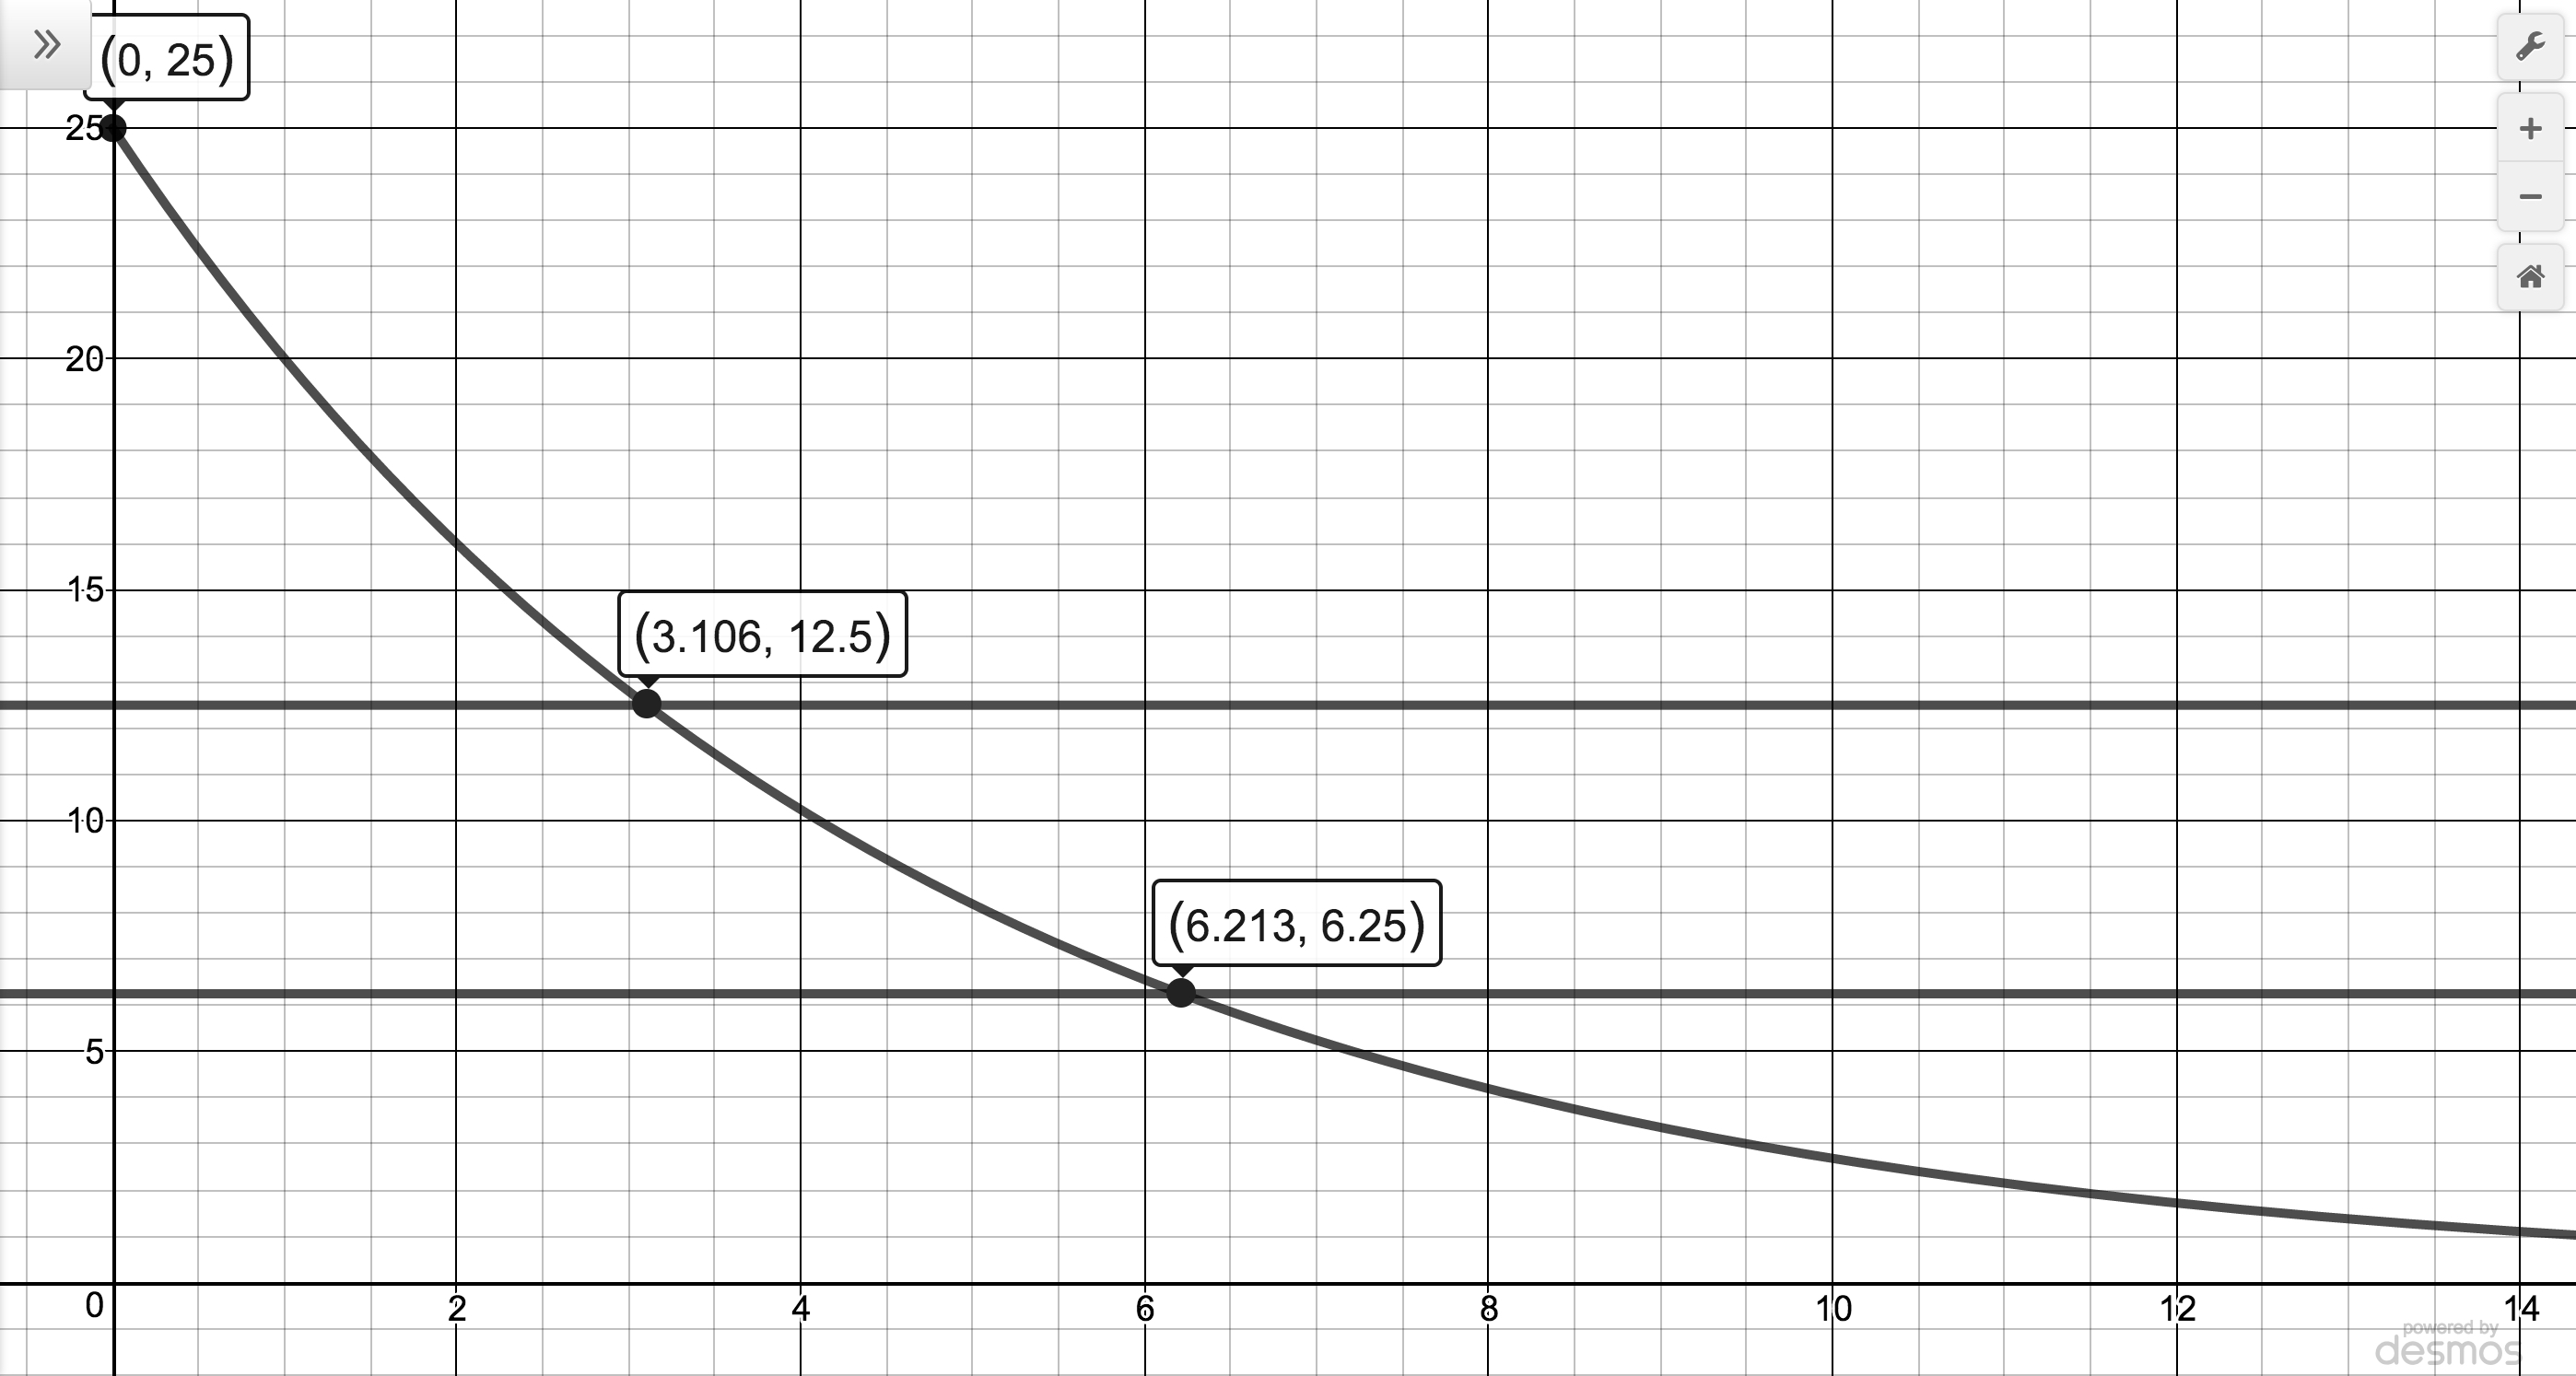
\includegraphics[width=6in]{./ExponentialFunctionsGraphics/ExponentialFunctionsEx01.jpg}

\end{center}

\qed
 
\end{enumerate}

\end{example}

Some remarks about Example \ref{cardepreciationex} are in order.  First the function in the previous example is  called a `decay curve'.  Increasing exponential functions are used to model `growth curves' and we shall see several different examples of those in Section \ref{ExpLogApplications}.  

\smallskip

Second, as seen in numbers \ref{georatio1} and \ref{georatio2},  $V(t+1) = 0.8 V(t)$.  That is to say, the function $V$ has a \textit{constant unit multiplier}, in this case, $0.8$ because to obtain the function value $V(t+1)$, we \textit{multiply} the function value $V(t)$ by $b$.   It is not coincidence that the multiplier here is the base of the exponential, $0.8$.

\smallskip

Indeed, exponential functions of the form $f(x) = a \cdot b^{x}$  have a constant unit multiplier, $b$.  To see this,  note \[ \dfrac{f(x+1)}{f(x)} = \dfrac{a \cdot b^{x+1}}{ a \cdot b^{x}} = b^{1} = b.\]

Hence $f(x+1) = f(x) \cdot b$.  This will prove useful to us in Section \ref{ExpLogApplications} when making decisions about whether or not a data set represents exponential growth or decay.  

\smallskip

More generally, one can show (see Exercise \ref{exponentialchangeexercise}) for any real number $x_{0}$ that $f(x_{0}+\Delta x) = f(x_{0}) b^{\Delta x}$. That is, to obtain $f(x_{0} + \Delta x)$ from $f(x_{0})$, we \textit{multiply} by $\Delta x$ factors of the constant unit multiplier, $b$.  This is at the heart of what it means to be an exponential function.

\smallskip

If this discussion seems familiar, it should.  For linear functions, $f(x) = mx +b$, we can obtain the slope $m$ by computing $f(x+1) - f(x)$.  To see this, note $f(x+1) - f(x)  = (m(x+1) +b) - (mx+b) = m$ so that $f(x+1) = f(x) + m$.  In this way, we see that the slope $m$ is the constant unit \textit{addend} in that in order to obtain $f(x+1)$, we \textit{add} $m$ to the function value $f(x)$.  

\smallskip

This notion is solidified in the point-slope form of a linear function,  Equation \ref{linearfunctionpointslope}.  For for any real numbers $x$ and $x_{0}$, we have   $f(x) = f(x_{0}) + m(x-x_{0})$.  If we let $x = x_{0}+ \Delta x$, we get $f(x_{0}+ \Delta x) = f(x_{0}) + m \Delta x$.  In other words, to obtain $f(x_{0}+\Delta x)$ from $f(x_{0})$, we \textit{add} $m$ times $\Delta x$. 

\smallskip

Taking inspiration from linear functions, we define the `point-base' form of an exponential function below.

\smallskip

%% \colorbox{ResultColor}{\bbm

\begin{definition} \label{expfcnpointbaseform}  The \index{exponential function ! point-base form} \index{point-base form ! of an exponential function} \textbf{point-base form} of the exponential function $f(x) = b^{x}$  is

\[ f(x) = f(x_{0}) b^{x - x_{0}} \]


\end{definition}

%% \ebm}

\smallskip

Just as the point-slope form of a linear function is helpful in building linear models, the point-base form of an exponential function will prove useful in building exponential models.

\smallskip

Next, while we saw in Example \ref{cardepreciationex} number \ref{cararcex}, exponential functions, unlike linear functions, do not have a constant rate of change.  However, in numbers \ref{carrelarcex1} and \ref{carrelarcex2}, we see that in some cases, they do have a constant \textit{relative} rate of change.  We define this notion below.

\smallskip


%% \colorbox{ResultColor}{\bbm

\begin{definition} \label{rrc}  Let $f$ be a function defined on the interval $[a,b]$ where $f(a) \neq 0$.

The \index{relative rate of change}\index{rate of change ! relative}\textbf{relative rate of  change}  of $f$ over $[a,b]$ is defined as: \[ \dfrac{\Delta [f(x)] }{f(a)} = \dfrac{f(b) - f(a)}{f(a)} .\]

\end{definition}

%% \ebm}

\smallskip

For exponential functions of the form $f(x) = a \cdot b^{x}$, we compute the relative rate of change over the interval $[x, x+1]$ and find it is constant:

\[ \dfrac{f(x+1) - f(x)}{f(x)} = \dfrac{f(x+1)}{f(x)} - \dfrac{f(x)}{f(x)} = b -1,\]

where we are using the fact that $\frac{f(x+1)}{f(x)} = b$. 

\smallskip

One way to interpret this result is when comparing $f(x)$ to $f(x+1)$, the exponential function grows (if $b>1$) or decays (if $b<1$) by $(b-1) \cdot 100 \%$.  In our example, $V(t) = 25 (0.8)^{t}$ so $b = 0.8$ and, as we saw, the relative rate of change from $V(t)$ to $V(t+1)$ was $ 0.8 - 1= -0.2$, meaning the value of the car  over the course of one year depreciates by  $20 \%$.

\smallskip

We close this section with another important application of exponential functions,  Newton's Law of Cooling.

\smallskip

\begin{example}  \label{exptempex} According to \href{http://en.wikipedia.org/wiki/Heat_transfer#Newton.27s_law_of_cooling}{\underline{Newton's Law of Cooling}}\footnote{We will discuss this in greater detail in Section \ref{ExpLogApplications}.} the temperature of coffee $T(t)$ (in degrees Fahrenheit) $t$ minutes after it is served can be modeled by $T(t) = 70 + 90 e^{-0.1 t}$. \index{Newton's Law of Cooling}

\begin{enumerate}

\item  Find and interpret $T(0)$.

\item  Sketch the graph of $y = T(t)$ using transformations.

\item  Find and interpret $\ds{\lim_{t \rightarrow \infty} T(t)}$.  

\end{enumerate}

{\bf Solution.}

\begin{enumerate}

\item  Since $T(0) =70 + 90 e^{-0.1 (0)} = 160$,   the temperature of the coffee when it is served is $160^{\circ}\mbox{F}$.

\item  To graph $y = T(t)$ using transformations, we start with the basic function, $f(t)=e^{t}$.  As in Example \ref{expfcngraphsex}, we track the points $(-1, e^{-1}) \approx (-1, 0.368)$, $(0,1)$, and $(1, e) \approx (1, 2.718)$, along wth the horizontal asymptote $y = 0$ through each of transformations.

\smallskip

To use Theorem  \ref{transformationsthm}, we rewrite   $T(t) = 70 + 90e^{-0.1t} = 90e^{-0.1t}+70 = 90 f(-0.1t)+70$.   Following Theorem  \ref{transformationsthm}, we first  divide the $t$-coordinates of each point on the graph of $y=f(t)$ by $-0.1$ which results in a horizontal expansion by a factor of $10$ as well as a reflection about the $y$-axis.  

\smallskip

Next, we multiply the $y$-values of the points on this new graph by $90$ which effects a vertical stretch by a factor of $90$.  Last but not least, we  add $70$ to all of the $y$-coordinates of the points on this second graph, which shifts the graph upwards $70$ units.


\smallskip


Tracking points, we have $(-1, e^{-1})  \rightarrow (10, e^{-1}) \rightarrow (10, 90e^{-1}) \rightarrow (10, 90e^{-1}+70) \approx (10, 103.112)$, $(0,1) \rightarrow (0,1) \rightarrow (0,90) \rightarrow (0, 160)$, and $(1,e) \rightarrow (-10, e) \rightarrow (-10, 90e) \rightarrow (-10, 90e+70) \approx (-10, 314.62)$.  The horizontal asymptote $y=0$ is unaffected by the horizontal expansion, reflection about the $y$-axis, and the vertical stretch.  The vertical shift moves the horizontal asymptote up $70$ units, $y = 0 \rightarrow y = 70$. After restricting the domain to $t \geq 0$, we get the graph below on the right.

\[\begin{array}{ccc}

\begin{mfpic}[15]{-4}{4}{-1}{8}
\axes
\tlabel[cc](-1,1){\scriptsize $(0,1)$}
\tlabel[cc](0,-1.5){\scriptsize H.A. $y=0$}
\tlabel[cc](4,-0.5){\scriptsize $t$}
\tlabel[cc](0.5,8){\scriptsize $y$}
\tcaption{\scriptsize $y = f(t)=e^{t}$}
\ymarks{1,2,3,4,5,6,7}
\xmarks{-3,-2,-1,1,2,3}
\tlpointsep{4pt}
\axislabels {x}{{\scriptsize $-3 \hspace{7pt}$} -3, {\scriptsize $-2 \hspace{7pt}$} -2, {\scriptsize $-1 \hspace{7pt}$} -1, {\scriptsize $1$} 1, {\scriptsize $2$} 2, {\scriptsize $3$} 3}
\axislabels {y}{{\scriptsize $2$} 2,{\scriptsize $3$} 3,{\scriptsize $4$} 4,{\scriptsize $5$} 5,{\scriptsize $6$} 6,{\scriptsize $7$} 7}
\penwd{1.25pt}
\arrow \reverse \arrow \function{-3, 2, 0.1}{exp(x)}
\point[4pt]{(0,1),(1,2.718), (-1,0.368)}
\end{mfpic}

&

\stackrel{\xrightarrow{\hspace{1in}}}{\text{\scriptsize Theorem  \ref{transformationsthm}}} 

&

\begin{mfpic}[15]{-1}{11}{-1}{10}
\dashed \polyline{(-1,3.5),(11,3.5)}
\axes
\tlabel[cc](9,2.5){\scriptsize H.A. $y=70$}
\tlabel[cc](11,-0.5){\scriptsize $t$}
\tlabel[cc](0.5,10){\scriptsize $y$}
\tlabel[cc](-1, 8){\scriptsize $(0, 160)$}
\tcaption{\scriptsize $y = T(t)$}
\ymarks{1,2,3,4,5,6,7,8,9}
\xmarks{1,2,3,4,5,6,7,8,9,10}
\tlpointsep{4pt}
\axislabels {x}{{\scriptsize $2$} 1, {\scriptsize $4$} 2, {\scriptsize $6$} 3, {\scriptsize $8$} 4,{\scriptsize $10$} 5, {\scriptsize $12$} 6, {\scriptsize $14$} 7, {\scriptsize $16$} 8, {\scriptsize $18$} 9, {\scriptsize $20$} 10}
\axislabels {y}{{\scriptsize $20$} 1, {\scriptsize $40$} 2, {\scriptsize $60$} 3,{\scriptsize $80$} 4, {\scriptsize $100$} 5, {\scriptsize $120$} 6,{\scriptsize $140$} 7, {\scriptsize $180$} 9}
\penwd{1.25pt}
\arrow \function{0, 10, 0.1}{(90*exp(0-0.2*x)+70)/20}
\point[4pt]{(0,8),(5,5.15)}
\end{mfpic} \\

\end{array}\]

\item  We can determine $\lim\limits_{t \rightarrow \infty} T(t)$ two ways.  First, we can employ  the `number sense' developed in Chapter \ref{RationalFunctions}.    

\smallskip

That is, as $t \rightarrow \infty$, We get $T(t) = 70+90e^{-0.1t} \approx 70 +90e^{\mbox{\scriptsize very big $(-)$}}$.  Since $e > 1$, $e^{\mbox{\scriptsize very big $(-)$}}  \approx \mbox{very small $(+)$}$  The larger $t$ becomes, the smaller $e^{-0.1t}$ becomes, so the term $90 e^{-0.1t} \approx \mbox{very small $(+)$}$.  Hence, $T(t) = 70+90e^{-0.1t}  \approx 70 +  \mbox{very small $(+)$} \approx 70$. 

\smallskip

Alternatively, we can look to the graph of $y = T(t)$.  We know the horizontal asymptote is $y=70$ which means as $t \rightarrow \infty$, $T(t) \approx 70$.

\smallskip

In either case, we find that as time goes by,  the temperature of the coffee is cooling to $70^{\circ}$ Fahrenheit, ostensibly room temperature. \qed

\end{enumerate}

\end{example}

\newpage

\subsection{Exercises}

%% SKIPPED %% \documentclass{ximera}

\begin{document}
	\author{Stitz-Zeager}
	\xmtitle{TITLE}
\mfpicnumber{1} \opengraphsfile{ExercisesforExponentialFunctions} % mfpic settings added 


\label{ExercisesforExponentialFunctions}



In Exercises \ref{graphexpfirsta} - \ref{graphexplasta}, sketch the graph of $g$ by starting with the graph of $f$ and using transformations.  Track at least three points of your choice and the horizontal asymptote through the transformations. State the domain and range of $g$.

\begin{multicols}{2}
\begin{enumerate}

\item  $f(x) = 2^{x}$, $g(x) = 2^{x} - 1$ \label{graphexpfirsta}

\item  $f(x) = \left(\frac{1}{3}\right)^{x}$, $g(x) = \left(\frac{1}{3}\right)^{x-1}$

\setcounter{HW}{\value{enumi}}
\end{enumerate}
\end{multicols}

\begin{multicols}{2}
\begin{enumerate}
\setcounter{enumi}{\value{HW}}

\item  $f(x) = 3^{x}$, $g(x) = 3^{-x}+2$

\item  $f(x) = 10^{x}$, $g(x) = 10^{\frac{x+1}{2}} - 20$  

\setcounter{HW}{\value{enumi}}
\end{enumerate}
\end{multicols}

\begin{multicols}{2}
\begin{enumerate}
\setcounter{enumi}{\value{HW}}

\item  $f(t) = (0.5)^{t}$, $g(t) = 100(0.5)^{0.1t}$

\item  $f(t) = (1.25)^{t}$, $g(t) = 1 - (1.25)^{t-2}$

\setcounter{HW}{\value{enumi}}
\end{enumerate}
\end{multicols}

\begin{multicols}{2}
\begin{enumerate}
\setcounter{enumi}{\value{HW}}

\item  $f(t) = e^{t}$, $g(t) = 8 - e^{-t}$

\item  $f(t) = e^{t}$, $g(t) = 10e^{-0.1t}$ \label{graphexplasta}

\setcounter{HW}{\value{enumi}}
\end{enumerate}
\end{multicols}

In Exercises, \ref{expformfirsta} - \ref{expformlasta}, the graph of an exponential function is given.  Find a formula for the function in the form $F(x) = a \cdot 2^{bx-h}+k$.

\begin{multicols}{2}
\begin{enumerate}
\setcounter{enumi}{\value{HW}}

\item  \label{expformfirsta}  Points:  $\left(-2, -\frac{5}{2} \right)$,  $\left(-1, -2 \right)$, $\left(0, -1 \right)$, \\
Asymptote:  $y = -3$. \\

\begin{mfpic}[13]{-5}{3}{-4}{6}
\axes
\tlabel[cc](3,-0.5){\scriptsize $x$}
\tlabel[cc](0.5,6){\scriptsize $y$}
\xmarks{-4, -3,-2,-1,1,2}
\ymarks{-3, -2, -1, 1,2,3,4,5}
\tlpointsep{4pt}
\axislabels {x}{{\scriptsize $-4 \hspace{7pt}$} -4,{\scriptsize $-3 \hspace{7pt}$} -3, {\scriptsize $-2 \hspace{7pt}$} -2, {\scriptsize $-1 \hspace{7pt}$} -1, {\scriptsize $1$} 1, {\scriptsize $2$} 2}
\axislabels {y}{{\scriptsize $1$} 1, {\scriptsize $2$} 2, {\scriptsize $3$} 3, {\scriptsize $4$} 4, {\scriptsize $5$} 5, {\scriptsize $-1$} -1, {\scriptsize $-2$} -2, {\scriptsize $-3$} -3}
\dashed \polyline{(-5,-3), (3,-3)}
\penwd{1.25pt}
\arrow \reverse \arrow \function{-4.5, 2.1, 0.1}{(2**(x+1))-3}
\point[4pt]{(-2, -2.5), (-1,-2),(0,-1)}
\end{mfpic}

\vfill

\columnbreak

\item  Points:  $\left(-1, 1 \right)$, $\left(0, 2 \right)$, $\left(1, \frac{5}{2} \right)$, \\
Asymptote:  $y = 3$. \\

\begin{mfpic}[13]{-4}{4}{-6}{4}
\axes
\tlabel[cc](4,-0.5){\scriptsize $x$}
\tlabel[cc](0.5,4){\scriptsize $y$}
\xmarks{-3,-2,-1,1,2,3}
\ymarks{-5 step 1 until 3}
\tlpointsep{4pt}
\axislabels {x}{{\scriptsize $-3 \hspace{7pt}$} -3, {\scriptsize $-2 \hspace{7pt}$} -2, {\scriptsize $-1 \hspace{7pt}$} -1, {\scriptsize $1$} 1, {\scriptsize $2$} 2, {\scriptsize $3$} 3}
\axislabels {y}{{\scriptsize $1$} 1, {\scriptsize $2$} 2, {\scriptsize $3$} 3, {\scriptsize $-1$} -1, {\scriptsize $-2$} -2, {\scriptsize $-3$} -3, {\scriptsize $-4$} -4, {\scriptsize $-5$} -5}
\dashed \polyline{(-4,3), (4,3)}
\penwd{1.25pt}
\arrow \reverse \arrow \function{-3, 3.1, 0.1}{3-(2**(-x))}
\point[4pt]{(-1,1), (0,2), (1, 2.5)}
\end{mfpic}



\setcounter{HW}{\value{enumi}}
\end{enumerate}
\end{multicols}

\begin{multicols}{2}
\begin{enumerate}
\setcounter{enumi}{\value{HW}}

\item  Points:  $\left(\frac{5}{2}, \frac{1}{2} \right)$, $\left(3,1 \right)$, $\left(\frac{7}{2}, 2 \right)$, \\
Asymptote:  $y = 0$. \\

\begin{mfpic}[13]{-1}{5}{-1}{9}
\axes
\tlabel[cc](5,-0.5){\scriptsize $x$}
\tlabel[cc](0.5,9){\scriptsize $y$}
\xmarks{1 step 1 until 4}
\ymarks{1 step 1 until 8}
\tlpointsep{4pt}
\axislabels {x}{{\scriptsize $1$} 1, {\scriptsize $2$} 2, {\scriptsize $3$} 3, {\scriptsize $4$} 4}
\axislabels {y}{{\scriptsize $1$} 1, {\scriptsize $2$} 2, {\scriptsize $3$} 3, {\scriptsize $4$} 4, {\scriptsize $5$} 5, {\scriptsize $6$} 6, {\scriptsize $7$} 7, {\scriptsize $8$} 8}
\penwd{1.25pt}
\arrow \reverse \arrow \function{1.25, 4.55, 0.1}{2**(2*x-6)}
\point[4pt]{(2.5, 0.5), (3,1), (3.5,2) }
\end{mfpic}

\vfill

\columnbreak

\item  Points:  $\left(-\frac{1}{2}, 6 \right)$, $\left(0,3 \right)$, $\left(\frac{1}{2}, \frac{3}{2} \right)$, \\
Asymptote:  $y = 0$.   \\

\begin{mfpic}[13]{-4}{4}{-1}{9}
\axes
\tlabel[cc](4,-0.5){\scriptsize $x$}
\tlabel[cc](0.5,9){\scriptsize $y$}
\xmarks{-3,-2,-1,1,2,3}
\ymarks{1,2,3,4,5,6,7,8}
\tlpointsep{4pt}
\axislabels {x}{{\scriptsize $-3 \hspace{7pt}$} -3, {\scriptsize $-2 \hspace{7pt}$} -2, {\scriptsize $-1 \hspace{7pt}$} -1, {\scriptsize $1$} 1, {\scriptsize $2$} 2, {\scriptsize $3$} 3}
\axislabels {y}{{\scriptsize $1$} 1, {\scriptsize $2$} 2, {\scriptsize $3$} 3,  {\scriptsize $7$} 7, {\scriptsize $8$} 8}
\penwd{1.25pt}
\arrow \reverse \arrow \function{-0.79, 2, 0.1}{3*(2**(-2*x))}
\point[4pt]{(-0.5, 6), (0,3), (0.5, 1.5)}
\end{mfpic}


\label{expformlasta} 

\setcounter{HW}{\value{enumi}}
\end{enumerate}
\end{multicols}


\begin{enumerate}
\setcounter{enumi}{\value{HW}}


\item 

Find a formula for each graph in Exercises \ref{expformfirsta} - \ref{expformlasta} of the form $G(x) = a \cdot 4^{bx-h} + k$.
  Did you change your solution methodology?    What is the relationship between your answers for $F(x)$ and $G(x)$ for each graph?

\item \label{morethanoneforexpexercise} In Example \ref{expfcngraphsex} number \ref{findformulaforexpexample}, we obtained the solution  $F(x) = -2^{x+3} + 4$ as one formula for the given graph by making a simplifying assumption that $a = -1$.  This exercises explores if there are any other solutions for different choices of $a$.

\begin{enumerate}

\item  Show  $G(x) = -4 \cdot 2^{x+1} + 4$ also fits the data for the given graph, and use  properties of exponents to show $G(x) = F(x)$.  (Use the fact that $4 = 2^2$ \ldots)

\item With help from your classmates, find solutions to  Example \ref{expfcngraphsex} number \ref{findformulaforexpexample} using $a = -8$, $a = -16$ and  $a = -\frac{1}{2}$.  Show all your solutions can be rewritten as: $F(x) = -2^{x+3} + 4$.

\item  Using properties of exponents and the fact that the range of $2^{x}$ is $(0, \infty)$, show that any function of the form $f(x) = -a \cdot 2^{bx-h} + k$ for $a> 0$ can be rewritten as $f(x) = - 2^{c} \, 2^{bx-h} + k = -2^{bx-h+c} + k$.  Relabeling, this means every function of the form $f(x) = -a \cdot 2^{bx-h} + k$ with four parameters ($a$, $b$, $h$, and $k$) can be rewritten as $f(x) =  - 2^{bx - H} + k$, a formula with just three parameters:  $b$, $H$, and $k$.  Conclude that  \textit{every} solution to Example \ref{expfcngraphsex} number \ref{findformulaforexpexample} reduces to $F(x) = -2^{x+3} + 4$ .

\end{enumerate}
\setcounter{HW}{\value{enumi}}
\end{enumerate}

In Exercises \ref{decomposebasicexpfirst} - \ref{decomposebasicexplast}, write the given function as a nontrivial decomposition of functions as directed.

\begin{enumerate}
\setcounter{enumi}{\value{HW}}

\item  For $f(x) = e^{-x} +1 $, find functions $g$ and $h$ so that $f=g+h$. \label{decomposebasicexpfirst}
\item  For $f(x) = e^{2x} - x$, find functions $g$ and $h$ so that $f=g-h$. 
\item  For $f(t) = t^2 e^{-t}$, find functions $g$ and $h$ so that $f=gh$.
\item  For $r(x) = \dfrac{e^{x} - e^{-x}}{e^{x}+e^{-x}}$, find functions $f$ and $g$ so $r = \dfrac{f}{g}$.
\item  For $k(x) = e^{-x^2}$, find functions $f$ and $g$  so that $k = g \circ f$.
\item  For $s(x) =\sqrt{e^{2x} - 1}$, find functions $f$ and $g$ so $s = g \circ f$. \label{decomposebasicexplast}


\item \label{preludetocompoundingexercise} The amount of money in a savings account, $A(t)$, in dollars,  $t$ years after an initial investment is made is given by: $A(t) = 500(1.05)^{t}$, for $t \geq 0$.

\begin{enumerate}

\item  Find and interpret $A(0)$, $A(1)$, and $A(2)$.  

\item  Find and interpret the relative rate of change of $A$ over the intervals $[0,1]$, $[1,2]$, $[0,2]$.

\item  Find, simplify, and interpret the relative rate of change of $A$ over the $[t, t+1]$.  Assume  $t \geq 0$.

\item Use a graphing utility to estimate how long until the savings account is worth $\$1500$.  Round your answer to the nearest year.

\end{enumerate}

\pagebreak

\item  Based on census data,\footnote{See \href{http://www.towncharts.com/Ohio/Demographics/Lake-County-OH-Demographics-data.html}{\underline{here}}.} the population of Lake County, Ohio, in 2010 was 230,041 and in 2015, the population was 229,437.  

\begin{enumerate}

\item  Show the percentage change in the population from 2010 to 2015 is approximately $-0.263 \%$.

\item  If this percentage change remains constant, predict the population of Lake County in 2020.

\item  \label{populationfiveyear} Assuming this percentage change per five years remains constant, find an expression for the population $P(t)$ of Lake County where $t$ is the number of five year intervals after 2010.  (So $t = 0$ corresponds to 2010, $t = 1$ corresponds to $2015$, $t = 2$ corresponds to $2020$, etc.)

HINT:  Definitions \ref{expfcnpointbaseform} and \ref{rrc} and ensuing discussion on that page is useful here.

\item  Use your answer to  \ref{populationfiveyear}  to predict the population of Lake County in the year 2017.  

\item  Let $A(t)$  represent the population of Lake County $t$ years after 2010 where the we approximate the percentage change in population per year as $-\frac{0.263 \%}{5} = -0.0526 \%$.    Find a formula for $A(t)$ and compare your predictions with $A(t)$ to those given by $P(t)$.  In particular, what population does each model give for the year 2050?  Discuss any discrepancies with your classmates.

\end{enumerate}


\item \label{averageofarc}  Show that the average rate of change of a function over the interval  $[x, x+2]$ is average of the average rates of change of the function over the intervals $[x,x+1]$ and $[x+1, x+2]$.  Can the same be said for the average rate of change of the function over $[x, x+3]$ and the average of the average rates of change over $[x, x+1]$, $[x+1, x+2]$, and $[x+2, x+3]$?  Generalize.

\item \label{exponentialchangeexercise}  If $f(x) = b^{x}$ where $b>0$, $b \neq 1$,  show $f(x_{0}+\Delta x) = f(x_{0}) b^{\Delta x}$.


\item Which is larger: $e^{\pi}$ or $\pi^{e}$?  How do you know?  Can you find a proof that doesn't use technology?


\item\label{derivativeofex} \begin{enumerate}  \item\label{diffquotex}  Use properties of exponential functions to show that if $f(x) = e^{x}$, then \[ f'(x) = \lim_{h \rightarrow 0} \frac{f(x+h) - f(x)}{h} = \lim_{h \rightarrow 0} e^{x} \, \left( \frac{e^{h} - 1}{h} \right)\]

\item\label{specialexlimit}    Numerically and graphically investigate the limit: $\ds{\lim_{h \rightarrow 0}}$ $\frac{e^{h} - 1}{h}$.

\item  Use parts \ref{diffquotex} and \ref{specialexlimit} to show to your surprise and delight that the derivative of $e^{x}$ is \ldots  $e^{x}$.

\item  Write the equations of the tangent lines to $y = e^{x}$ at the following points:

\begin{enumerate}

\item  $(0,1)$

\item  $(1, e)$

\item $\left(-1, e^{-1} \right)$

\end{enumerate}

\end{enumerate}

\setcounter{HW}{\value{enumi}}
\end{enumerate}


\newpage

\subsection{Answers}

\begin{multicols}{2}
\begin{enumerate}


\item  Domain of $g$:  $(-\infty, \infty)$\\
 Range of $g$:  $(-1, \infty)$\\
 Points:  $\left(-1, -\frac{1}{2} \right)$, $(0,0)$, $(1,1)$\\
Asymptote: $y = -1$\\
 
\begin{mfpic}[15]{-4}{4}{-2}{9}
\point[4pt]{(-1,-0.5), (0,0), (1,1)}
\axes
\tlabel[cc](4,-0.5){\scriptsize $x$}
\tlabel[cc](0.5,9){\scriptsize $y$}
\tcaption{$y = g(x) = 2^{x}-1$}
\xmarks{-3,-2,-1,1,2,3}
\ymarks{-1,1,2,3,4,5,6,7,8}
\tlabel[cc](-3,0.5){\tiny $-3 \hspace{7pt}$}
\tlabel[cc](-2,0.5){\tiny $-2 \hspace{7pt}$}
\tlabel[cc](-1,0.5){\tiny $-1 \hspace{7pt}$}
\tlpointsep{4pt}
\axislabels {x}{{\tiny $1$} 1, {\tiny $2$} 2, {\tiny $3$} 3}
\axislabels {y}{{\tiny $1$} 1, {\tiny $2$} 2, {\tiny $3$} 3, {\tiny $4$} 4, {\tiny $5$} 5, {\tiny $6$} 6, {\tiny $7$} 7, {\tiny $8$} 8}
\dashed \polyline{(-4,-1),(4,-1)}
\penwd{1.25pt}
\arrow \reverse \arrow \function{-3.5, 3.1, 0.1}{(2**(x))-1}
\end{mfpic}

\vfill

\columnbreak

\item  Domain of $g$:  $(-\infty, \infty)$ \\
 Range of $g$:  $(0, \infty)$ \\
  Points:  $(0,3)$, $(1,1)$, $\left(2, \frac{1}{3} \right)$\\
 Asymptote: $y = 0$\\
 
\begin{mfpic}[15]{-4}{4}{-1}{10}
\point[4pt]{(0,3), (1,1), (2,0.3333)}
\axes
\tlabel[cc](4,-0.5){\scriptsize $x$}
\tlabel[cc](0.5,10){\scriptsize $y$}
\tcaption{$y = g(x) = \left(\frac{1}{3}\right)^{x-1}$}
\xmarks{-3,-2,-1,1,2,3}
\ymarks{1,2,3,4,5,6,7,8,9}
\tlpointsep{4pt}
\axislabels {x}{{\tiny $-3 \hspace{7pt}$} -3, {\tiny $-2 \hspace{7pt}$} -2, {\tiny $-1 \hspace{7pt}$} -1, {\tiny $1$} 1, {\tiny $2$} 2, {\tiny $3$} 3}
\axislabels {y}{{\tiny $1$} 1, {\tiny $2$} 2, {\tiny $3$} 3, {\tiny $4$} 4, {\tiny $5$} 5, {\tiny $6$} 6, {\tiny $7$} 7, {\tiny $8$} 8, {\tiny $9$} 9}
\penwd{1.25pt}
\arrow \reverse \arrow \function{-1.05, 3.5, 0.1}{3**(1-x)}
\end{mfpic} 

\setcounter{HW}{\value{enumi}}
\end{enumerate}
\end{multicols}

\begin{multicols}{2}
\begin{enumerate}
\setcounter{enumi}{\value{HW}}

\item  Domain of $g$:  $(-\infty, \infty)$\\
 Range of $g$:  $(2, \infty)$\\
  Points:  $\left(1, \frac{7}{3} \right)$, $(0,3)$, $(-1,5)$\\
  Asymptote:  $y = 2$ \\

\begin{mfpic}[15]{-4}{4}{-1}{12}
\point[4pt]{(1,2.3333), (0,3), (-1,5)}
\axes
\tlabel[cc](4,-0.5){\scriptsize $x$}
\tlabel[cc](0.5,12){\scriptsize $y$}
\tcaption{$y = g(x) = 3^{-x}+2$}
\xmarks{-3,-2,-1,1,2,3}
\ymarks{1,2,3,4,5,6,7,8,9,10,11}
\tlpointsep{4pt}
\axislabels {x}{{\tiny $-3 \hspace{7pt}$} -3, {\tiny $-2 \hspace{7pt}$} -2, {\tiny $-1 \hspace{7pt}$} -1, {\tiny $1$} 1, {\tiny $2$} 2, {\tiny $3$} 3}
\axislabels {y}{{\tiny $1$} 1, {\tiny $2$} 2, {\tiny $3$} 3, {\tiny $4$} 4, {\tiny $5$} 5, {\tiny $6$} 6, {\tiny $7$} 7, {\tiny $8$} 8, {\tiny $9$} 9, {\tiny $10$} 10, {\tiny $11$} 11}
\dashed \polyline{(-4,2),(4,2)}
\penwd{1.25pt}
\arrow \reverse \arrow \function{-2.05, 2.5, 0.1}{2+3**(0-x)}
\end{mfpic}

\vfill

\columnbreak

\item  Domain of $g$:  $(-\infty, \infty)$\\
 Range of $g$:  $(-20, \infty)$\\
  Points:  $\left(-1,-19 \right)$, $(1,-10)$, $(3,80)$\\
  Asymptote:  $y = -20$\\
 
\begin{mfpic}[15]{-3}{4}{-2}{9}
\point[4pt]{(-1,-1.9), (1,-1), (3,8)}
\axes
\tlabel[cc](4,-0.5){\scriptsize $x$}
\tlabel[cc](0.5,9){\scriptsize $y$}
\tcaption{$y = g(x) = 10^{\frac{x+1}{2}}-20$}
\xmarks{-3,-2,-1,1,2,3}
\ymarks{-2,-1,1,2,3,4,5,6,7,8}
\tlpointsep{4pt}
\axislabels {x}{{\tiny $-3 \hspace{7pt}$} -3, {\tiny $-2 \hspace{7pt}$} -2,  {\tiny $1$} 1, {\tiny $2$} 2, {\tiny $3$} 3}
\axislabels {y}{{\tiny $-10$} -1,{\tiny $10$} 1, {\tiny $20$} 2, {\tiny $30$} 3, {\tiny $40$} 4, {\tiny $50$} 5, {\tiny $60$} 6, {\tiny $70$} 7, {\tiny $80$} 8}
\dashed \polyline{(-4,-2), (4,-2)}
\penwd{1.25pt}
\arrow \reverse \arrow \function{-3, 3.06, 0.1}{((10**((x+1)/2))-20)/10}
\end{mfpic}

\setcounter{HW}{\value{enumi}}
\end{enumerate}
\end{multicols}

\begin{multicols}{2}
\begin{enumerate}
\setcounter{enumi}{\value{HW}}

\item  Domain of $g$:  $(-\infty, \infty)$\\
  Range of $g$:  $(0, \infty)$ \\
  Points:  $(-10, 200)$, $(0, 100)$, $(10, 50)$\\
  Asymptote: $y = 0$\\
 
\begin{mfpic}[15]{-4}{4}{-1}{9}
\point[4pt]{(-1,2), (0,1), (1, 0.5)}
\axes
\tlabel[cc](4,-0.5){\scriptsize $t$}
\tlabel[cc](0.5,9){\scriptsize $y$}
\tcaption{ $y = g(t) = 100(0.5)^{0.1t}$}
\xmarks{-3,-2,-1,1,2,3}
\ymarks{1,2,3,4,5,6,7,8}
\tlpointsep{4pt}
\axislabels {x}{{\tiny $-30 \hspace{7pt}$} -3, {\tiny $-20 \hspace{7pt}$} -2, {\tiny $-10 \hspace{7pt}$} -1, {\tiny $10$} 1, {\tiny $20$} 2, {\tiny $30$} 3}
\axislabels {y}{{\tiny $100$} 1, {\tiny $200$} 2, {\tiny $300$} 3, {\tiny $400$} 4, {\tiny $500$} 5, {\tiny $600$} 6, {\tiny $700$} 7, {\tiny $800$} 8}
\penwd{1.25pt}
\arrow \reverse \arrow \function{-3, 3, 0.1}{0.5**x}
\end{mfpic}

\vfill

\columnbreak


\item  Domain of $g$:  $(-\infty, \infty)$\\
  Range of $g$:  $(-\infty, 1)$ \\
  Points:  $(1, 0.2)$, $(2,0)$, $(3,-0.25)$\\
  Asymptote: $y = 1$\\
 
\begin{mfpic}[10][8]{-8}{5}{-11}{11}
\point[4pt]{(1,2), (2,0), (3, -2.5)}
\axes
\tlabel[cc](5,-0.5){\scriptsize $t$}
\tlabel[cc](0.5,11){\scriptsize $y$}
\tcaption{ $y = g(t) = 1-(1.25)^{t-2}$}
\xmarks{-8 step 1 until 4}
\ymarks{-10 step 1 until 10}
\tlpointsep{4pt}
\axislabels {x}{{\tiny $-8 \hspace{7pt}$} -8,{\tiny $-6 \hspace{7pt}$} -6,{\tiny $-4 \hspace{7pt}$} -4,{\tiny $-2 \hspace{7pt}$} -2, {\tiny $2$} 2, {\tiny $4$} 4}
\axislabels {y}{ {\tiny $0.2$} 2,  {\tiny $0.4$} 4,  {\tiny $0.6$} 6, {\tiny $0.8$} 8, {\tiny $1$} 10, {\tiny $-0.2$} -2, {\tiny $-0.4$} -4,  {\tiny $-0.6$} -6, {\tiny $-0.8$} -8, {\tiny $-1$} -10}
 
\dashed \polyline{(-8, 10), (5, 10)}
\penwd{1.25pt}
\arrow \reverse \arrow \function{-8, 5, 0.1}{(1- (1.25**(x-2)))*10}
\end{mfpic}

\setcounter{HW}{\value{enumi}}
\end{enumerate}
\end{multicols}



\begin{multicols}{2}
\begin{enumerate}
\setcounter{enumi}{\value{HW}}

\item  Domain of $g$:  $(-\infty, \infty)$\\
 Range of $g$:  $(-\infty, 8)$ \\
  Points:  $\left(1, 8-e^{-1} \right) \approx (1, 7.63)$,  \\
  $(0,7)$, $\left(-1,  8-e \right) \approx (1,5.28) $\\
 Asymptote:  $y = 8$ \\
 
\begin{mfpic}[15]{-4}{4}{-1}{9}
\point[4pt]{(1,7.6321), (0,7), (-1,5.282)}
\axes
\tlabel[cc](4,-0.5){\scriptsize $t$}
\tlabel[cc](0.5,9){\scriptsize $y$}
\tcaption{ $y = g(t) = 8-e^{-t}$}
\xmarks{-3,-2,-1,1,2,3}
\ymarks{1,2,3,4,5,6,7,8}
\tlpointsep{4pt}
\axislabels {x}{{\tiny $-3 \hspace{7pt}$} -3, {\tiny $-2 \hspace{7pt}$} -2, {\tiny $-1 \hspace{7pt}$} -1, {\tiny $1$} 1, {\tiny $2$} 2, {\tiny $3$} 3}
\axislabels {y}{{\tiny $1$} 1, {\tiny $2$} 2, {\tiny $3$} 3, {\tiny $4$} 4, {\tiny $5$} 5, {\tiny $6$} 6, {\tiny $7$} 7, {\tiny $8$} 8}
\dashed \polyline{(-4,8), (4,8)}
\penwd{1.25pt}
\arrow \reverse \arrow \function{-2.25, 2, 0.1}{8-exp(0-x)}
\end{mfpic}

\vfill

\columnbreak


\item  Domain of $g$:  $(-\infty, \infty)$\\
 Range of $g$:  $(0, \infty)$\\
 Points:  $\left(10, 10e^{-1} \right) \approx (10, 3.68)$ \\
 $(0,10)$, $\left(-10, 10e \right) \approx (-10, 27.18)$  \\
 Asymptote:  $y = 0$\\
 
\begin{mfpic}[15]{-4}{4}{-1}{9}
\point[4pt]{(1,0.3679), (0,1), (-1,2.718)}
\axes
\tlabel[cc](4,-0.5){\scriptsize $t$}
\tlabel[cc](0.5,9){\scriptsize $y$}
\tcaption{$y = g(t) = 10e^{-0.1t}$}
\xmarks{-3,-2,-1,1,2,3}
\ymarks{1,2,3,4,5,6,7,8}
\tlpointsep{4pt}
\axislabels {x}{{\tiny $-10 \hspace{7pt}$} -1, {\tiny $10$} 1, {\tiny $20$} 2, {\tiny $30$} 3}
\axislabels {y}{{\tiny $10$} 1, {\tiny $20$} 2, {\tiny $30$} 3, {\tiny $40$} 4, {\tiny $50$} 5, {\tiny $60$} 6, {\tiny $70$} 7, {\tiny $80$} 8}
\penwd{1.25pt}
\arrow \reverse \arrow \function{-2.15, 2, 0.1}{exp(0-x)}
\end{mfpic}

\setcounter{HW}{\value{enumi}}
\end{enumerate}
\end{multicols}

\begin{multicols}{4}
\begin{enumerate}
\setcounter{enumi}{\value{HW}}

\item $F(x) = 2^{x+1}-3$

\item  $F(x) = -2^{-x} + 3$

\item $F(x) = 2^{2x-6}$

\item  $F(x) =3 \cdot 2^{-2x}$

\setcounter{HW}{\value{enumi}}
\end{enumerate}
\end{multicols}

\begin{enumerate}
\setcounter{enumi}{\value{HW}}

\item  Since $2 = 4^{\frac{1}{2}}$, one way to obtain the formulas for $G(x)$ is to use properties of exponents.  For example, $F(x) = 2^{x+1}-3 = \left(4^{\frac{1}{2}}\right)^{x+1} -3 = 4^{\frac{1}{2}(x+1)} - 3 = 4^{\frac{1}{2} x + \frac{1}{2}} - 3$.  In order, the formulas for $G(x)$ are:

\begin{multicols}{4}
\begin{itemize}

\item $G(x) = 4^{\frac{1}{2}x+\frac{1}{2}}-3$

\item  $G(x) = -4^{-\frac{1}{2} x} + 3$

\item $G(x) = 4^{x-3}$

\item  $G(x) =3 \cdot 4^{-x}$

\end{itemize}
\end{multicols}

\setcounter{HW}{\value{enumi}}
\end{enumerate}

\begin{enumerate}
\setcounter{enumi}{\value{HW}}

\addtocounter{enumi}{1}

\begin{multicols}{2}

\item\footnote{Answers for Exercises \ref{decomposebasicexpfirst} - \ref{decomposebasicexplast} vary.  We list one solution for each problem.}$g(x)  = e^{-x}$ and $h(x) = 1$.
\item $g(x) = e^{2x}$ and $h(x) = x$.

\end{multicols}

\setcounter{HW}{\value{enumi}}
\end{enumerate}

\begin{enumerate}
\setcounter{enumi}{\value{HW}}

\begin{multicols}{2}

\item   $g(t) = t^2$ and $h(t) = e^{-t}$.
\item   $f(x) = e^{x} - e^{-x}$ and $g(x) = e^{x}+e^{-x}$.

\end{multicols}

\setcounter{HW}{\value{enumi}}
\end{enumerate}

\begin{enumerate}
\setcounter{enumi}{\value{HW}}

\begin{multicols}{2}
\item   $f(x) = -x^2$ and $g(x) = e^{x}$.
\item   $f(x) = e^{2x} -1$ and $g(x) = \sqrt{x}$.  
\end{multicols}

\setcounter{HW}{\value{enumi}}
\end{enumerate}

\begin{enumerate}
\setcounter{enumi}{\value{HW}}

\item  \begin{enumerate}

\item   $A(0) = 500$, so the principal is $\$500$.  $A(1) = 525$, so after $1$ year, there is $\$525$ in the savings account.   $A(2) =551.25$, so after $2$ years, there is $\$551.25$ in the savings account. 

\item  The relative rate of change of $A$ over the intervals $[0,1]$ and $[1,2]$ is $0.05$ which means the savings account is growing by $5 \%$ each year for those two years.  Over the interval $[0,2]$, the relative rate of change is $0.1025$ meaning the account has grown by $10.25 \%$ over the course of the first two years.  Note this is greater than the sum of the two rates $5 \% + 5 \% = 10 \%$.  This is due to the `compounding effect' and will be discussed in greater detail in Section \ref{ExpLogApplications}.

\item  The relative rate of change of $A$ over the $[t, t+1]$ is $0.05$. This means over the course of one year, the savings account grows by $5 \%$.

\item Graphing $y= A(t)$ and $y = 1500$, we find they intersect when $t \approx 22.5$ so it takes approximately $22-23$ years for the savings account to grow to $\$1500$ in value.

\end{enumerate}

\item  \begin{enumerate}

\item $\frac{229437-230041}{230041} \approx 0.263 \%$.

\item  Since 2020 is five years after 2015, we expect the population to decrease by  $0.263 \%$ of 229437, or approximately 603 people.  Hence, we approximate the population in 2020 as 228834.

\item  $P(t) = 230041(1-0.00263)^t = 230041(0.99737)^{t}$, $t \geq 0$.

\item  Since 2017 is 7 years after 2010, we set $t = \frac{7}{5} = 1.4$ and find $P(1.4) \approx 229194$.  So the population is approximately 229, 194 in 2017.  

\item  $A(t) = 230041(1 - 0.0005626)^{t} =  230041 (0.999474)^{t}$, $t \geq 0$.  Since 2050 is 40 years after 2010, using the model $P(t)$, we divide $\frac{40}{5} = 8$ and find $P(8) \approx 225,245$. On the other hand, $A(40) \approx 225,250$.  This is more than roundoff error.  There is a compounding effect which makes the functions $A(t)$ and $P(t)$ different. \footnote{See number \ref{preludetocompoundingexercise} above or, for more, see Section \ref{ExpLogApplications}.}

\end{enumerate}

\addtocounter{enumi}{3}

\enlargethispage{0.25in}

\item  \begin{enumerate}
\addtocounter{enumii}{3}

\item \begin{multicols}{3} \begin{enumerate} \item $y = x+1$ \item  $y = e \, x $  \item  $y = e^{-1} \, x + 2e^{-1}$  \end{enumerate}  \end{multicols} \end{enumerate}


\setcounter{HW}{\value{enumi}}
\end{enumerate}




\end{document}


\closegraphsfile

\end{document}
